\documentclass{article}

% Use numeric citations, compressing consecutive citations such as [2--5].
\PassOptionsToPackage{numbers,compress}{natbib}

% accepted paper, camera-ready version
\usepackage[final]{tackling_climate_workshop_style}

% to compile a preprint version, e.g., for submission to arXiv, add add the
% [preprint] option:
%     \usepackage[preprint]{tackling_climate_workshop_style}

% to compile a camera-ready version, add the [final] option, e.g.:
%     \usepackage[final]{tackling_climate_workshop_style}

% to avoid loading the natbib package, add option nonatbib (not used here):
% \usepackage[nonatbib]{tackling_climate_workshop_style}

\usepackage[utf8]{inputenc} % allow utf-8 input
\usepackage[T1]{fontenc}    % use 8-bit T1 fonts
\usepackage{hyperref}       % hyperlinks
\usepackage{url}            % simple URL typesetting
\usepackage{booktabs}       % professional-quality tables
\usepackage{graphicx}       % include figures
\usepackage{amsmath}        % mathematical typesetting
\usepackage{amsfonts}       % blackboard math symbols
\usepackage{nicefrac}       % compact symbols for 1/2, etc.
\usepackage{microtype}      % microtypography

\title{Run it Back: Autoregression vs. Video Diffusion for End-Conditioned Weather Trajectories}

% The \author macro works with any number of authors. There are two commands
% used to separate the names and addresses of multiple authors: \And and \AND.
%
% Using \And between authors leaves it to LaTeX to determine where to break the
% lines. Using \AND forces a line break at that point. So, if LaTeX puts 3 of 4
% authors names on the first line, and the last on the second line, try using
% \AND instead of \And before the third author name.

\author{Jerry Lin \\
  Department of Computing and Data Sciences \\
  Boston University \\
  Boston, MA 02215 \\
  \texttt{jlin404@bu.edu}
  \And
  Elizabeth A. Barnes \\
  Department of Computing and Data Sciences \\
  Boston University \\
  \texttt{eabarnes@bu.edu}
}

\begin{document}

\maketitle

\begin{abstract}

The severity of low-likelihood, high-impact (LLHI) extremes is projected to increase in a warming climate. Sampling the range of precursors that lead to these events traditionally requires massive ensembles that scale poorly with lead time and rarity. While specialized rare-event sampling and ensemble-boosting methods are emerging, they do not demonstrate how a \textit{single} extreme might arise from diverse synoptic precursors. \citet{Lin2026-sz} recently demonstrated this is possible using end-conditioned trajectories from a video diffusion climate emulator (cBottle-video), but the resulting ensembles were structurally underdispersed, geostrophically inconsistent, and over a fixed window length. Notably, cBottle-video was evaluated as an off-the-shelf multi-task checkpoint trained with general masked conditional video diffusion (MCVD) \citep{Brenowitz2025-mz, voleti2022MCVD}. Whether a dedicated reverse-time autoregressive model generates more physically credible backward trajectories remains an open question. Here, we train a backward-in-time probabilistic autoregressive model using a FourCastNet~3 backbone \citep{Bonev2025-dw} to generate systematically diverse, end-conditioned trajectories for two of these case studies. Although the approach is promising, rollout instability indicates that further refinement may be necessary.

\end{abstract}

\section{Introduction}

With a warming climate, humanity is likely to experience more severe heatwaves, droughts, hurricanes, and floods \citep{Domeisen2022-gj,Hirabayashi2013-ry, Knutson2020-tj, Fischer2025-na, IPCC2023Sections, Cook2020-xw}. Understanding how such events can unfold is critical for risk assessment and scenario planning, but traditionally requires generating large physics-based ensembles at high computational cost. Because large ensembles scale poorly with lead time and event rarity, emerging techniques such as ensemble boosting, initial-condition optimization, and rare-event sampling directly target stronger extremes without exhaustive search \citep{Ragone2018-rj, Gessner2021-qy, Finkel2024-ln, Finkel2026-uu, Whittaker2026-fe, Hakim2026-oy, Lancelin2026-om}. While useful, none of these techniques target how multiple diverse trajectories could lead to the \textit{same} event. For local stakeholders, however, identifying stronger extremes in isolation is insufficient; contingency planning requires characterizing a range of plausible antecedent pathways that may culminate in a specific regional disaster.

Recently, \citet{Lin2026-sz} used Climate in a Bottle-Video (cBottle-video), a video diffusion climate emulator, to generate 1,000-member ensembles that converge on a single extreme event across three case studies---the 2021 Pacific Northwest heatwave, Superstorm Sandy, and Hurricane Ian---achieving antecedent diversity comparable to start-conditioned ensembles. Because cBottle-video is trained using general-purpose masked conditioning over fixed 66-hour windows, this naturally raises the question: can a dedicated autoregressive architecture trained explicitly on reverse-time state transitions generate more physically credible backward trajectories? Here, we address this question by developing a backward-in-time probabilistic autoregressive model based on a FourCastNet~3 backbone \citep{Bonev2025-dw} trained directly for reverse-time rollout. Although the autoregressive rollouts exhibit dynamical instability over medium-range weather horizons, the generated backward trajectories demonstrate greater synoptic coherence and large-scale dynamical organization---with leading 500 hPa geopotential height ($z_{500}$) modes organizing antecedent heatwave temperatures and hurricane tracks more effectively than cBottle-video over its 66-hour context window.

\section{Methods}

\subsection{Backward-in-time probabilistic autoregressive model}

We configure a 273.5M-parameter FourCastNet~3 backbone as a probabilistic autoregressive model of the reverse-time conditional distribution $p(\mathbf{x}_{t-6\mathrm{h}}\mid\mathbf{x}_t)$ \citep{Bonev2025-dw}. The model is trained on 10 years of ERA5 reanalysis data (2009--2018, inclusive, with 2019 used for validation) on a regular $0.25^\circ$ latitude--longitude grid ($\sim$25\,km resolution) and generates multistep trajectories through autoregressive six-hour rollouts \citep{Hersbach2020-oh}. Full architecture, state representation, normalization, objective, and training details are provided in Supplementary Section~\ref{sec:methods_fcn3_backward}.

\subsection{Climate in a Bottle Video (cBottle-video)}
\label{sec:methods_cbottle_main}

cBottle-video is a score-based video diffusion model trained on 38 years of ERA5 reanalysis data (1980--2017, validated on 2018) regridded to an equal-area HEALPix grid ($\sim$100\,km resolution). It generates 66-hour (12-frame) trajectories simultaneously with the ability to arbitrarily condition on any subset of frames \citep{Brenowitz2025-mz, Lin2026-sz}. Case study results for this model are taken directly from \citet{Lin2026-sz}. Full architecture, masked-conditioning formulation, and ODE sampling details are described in \citet{Brenowitz2025-mz} and are additionally provided in Supplementary Section~\ref{sec:methods_cbottle}.

\section{Results}

\subsection{Hurricane Ian (2022)}

\begin{figure}[t]
\centering
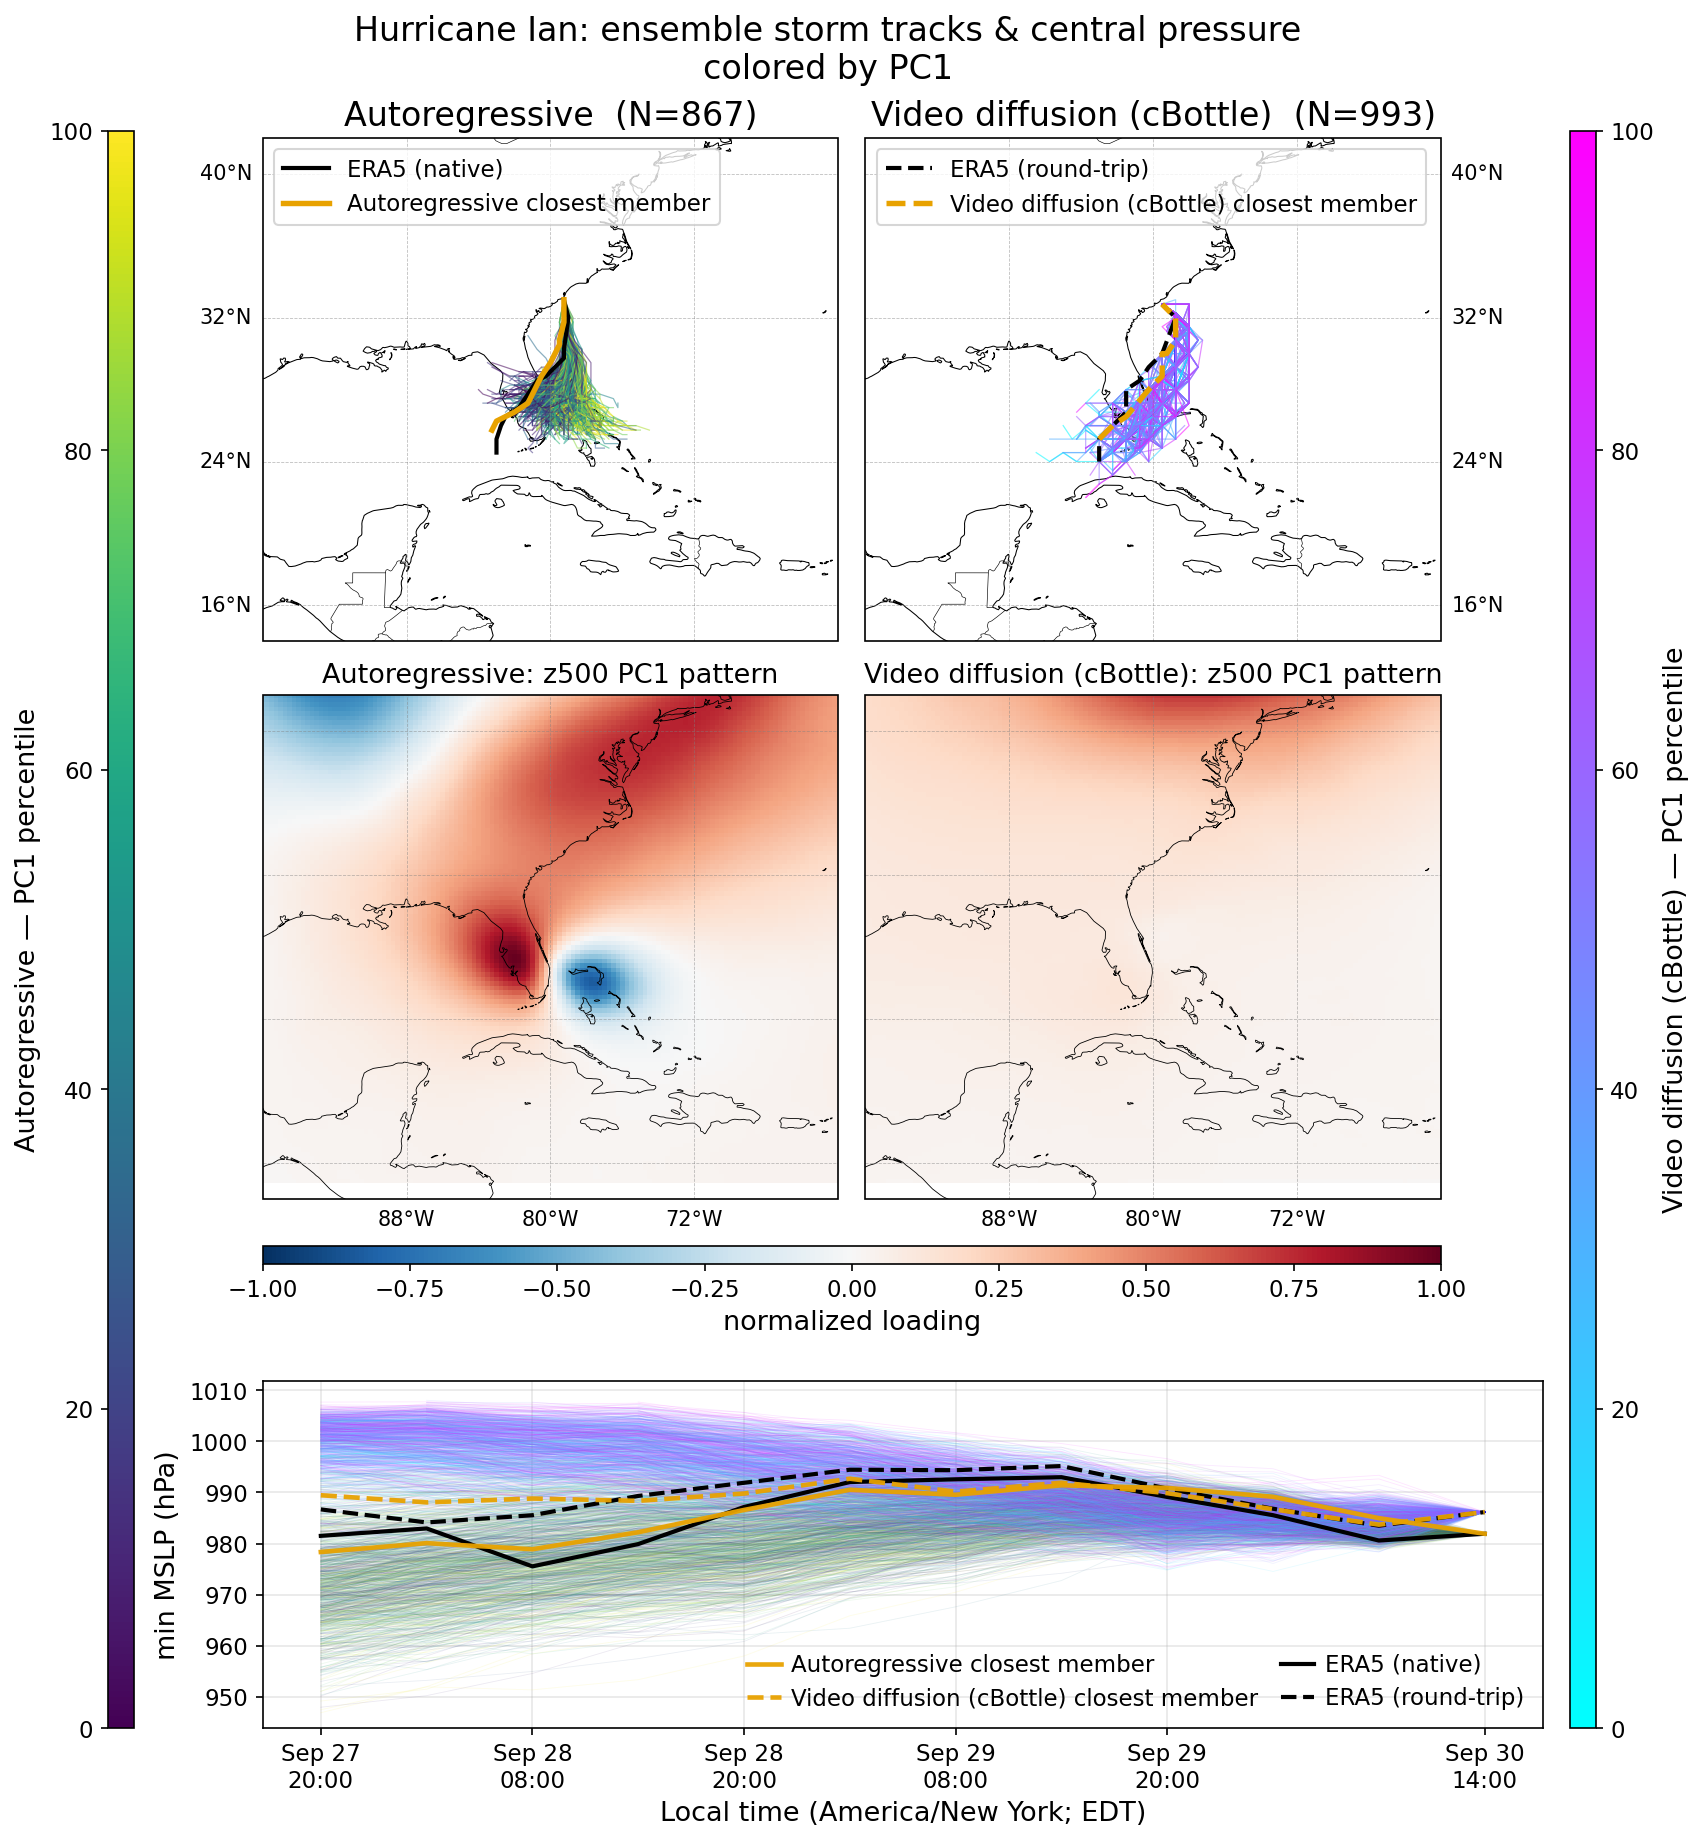
\includegraphics[width=\linewidth]{ian_tracks_intensity.png}
\caption{Hurricane Ian 66-hour end-conditioned ensemble comparison between the autoregressive model and cBottle-video. (Top) Storm tracks identified using TempestExtremes and colored by free-end $z_{500}$ PC1 percentile \citep{Ullrich2021-nm, Lin2026-sz}. (Middle) Normalized spatial loading patterns of the leading $z_{500}$ empirical orthogonal function (EOF1) computed over $110^{\circ}$--$50^{\circ}$~W, $15^{\circ}$--$50^{\circ}$~N at $t=0$. (Bottom) Evolution of minimum mean sea level pressure (MSLP, hPa) over local time (EDT) across ensemble members. The ensembles start with 1,000 members: the autoregressive results retain 867 after stability screening (all 1,000 pass track QC), while cBottle-video retains 993 after track QC (seven lack a qualifying Ian track). Highlighted members are retrospectively selected examples. ERA5 references are native-grid for the autoregressive model and HEALPix-round-tripped for cBottle-video.}
\label{fig:ian-tracks-intensity}
\end{figure}

Figure~\ref{fig:ian-tracks-intensity} compares 66-hour ensemble trajectories end-conditioned on ERA5 at the time of Hurricane Ian's South Carolina landfall (September 30, 2022, 18:00 UTC). In cBottle-video, the leading eight $z_{500}$ principal components show weak positive associations with free-end storm position, explaining approximately 7\% of in-sample and 5\% of cross-validated variance in free-end latitude, longitude, and distance from ERA5 (Supplementary Figure~\ref{fig:si-eof-regression-ian}), consistent with the weak association previously reported for cBottle-video \citep{Lin2026-sz}. In contrast, the autoregressive model's 867 stability-screened members (all 1,000 members pass Ian track QC) show stronger associations: the leading mode of $z_{500}$ variance (PC1) smoothly sorts antecedent tracks across the Florida peninsula and eastern Gulf of Mexico (Figure~\ref{fig:ian-tracks-intensity}, top left). The corresponding EOF1 spatial loading (Figure~\ref{fig:ian-tracks-intensity}, middle left) shows a coherent synoptic dipole---an anomalous mid-tropospheric ridge over the southeastern United States paired with an offshore trough southeast of Florida---consistent with synoptic steering, alongside the more diffuse cBottle-video loading.

Some autoregressive members reach central pressures below 960\,hPa (Figure~\ref{fig:ian-tracks-intensity}, bottom). The highlighted trajectories are retrospectively selected examples.

Regression diagnostics relating the leading eight free-end $z_{500}$ principal components to storm position and intensity are shown in Supplementary Figure~\ref{fig:si-eof-regression-ian}. 

\subsection{2021 Pacific Northwest heatwave}

\begin{figure}[t]
  \centering
  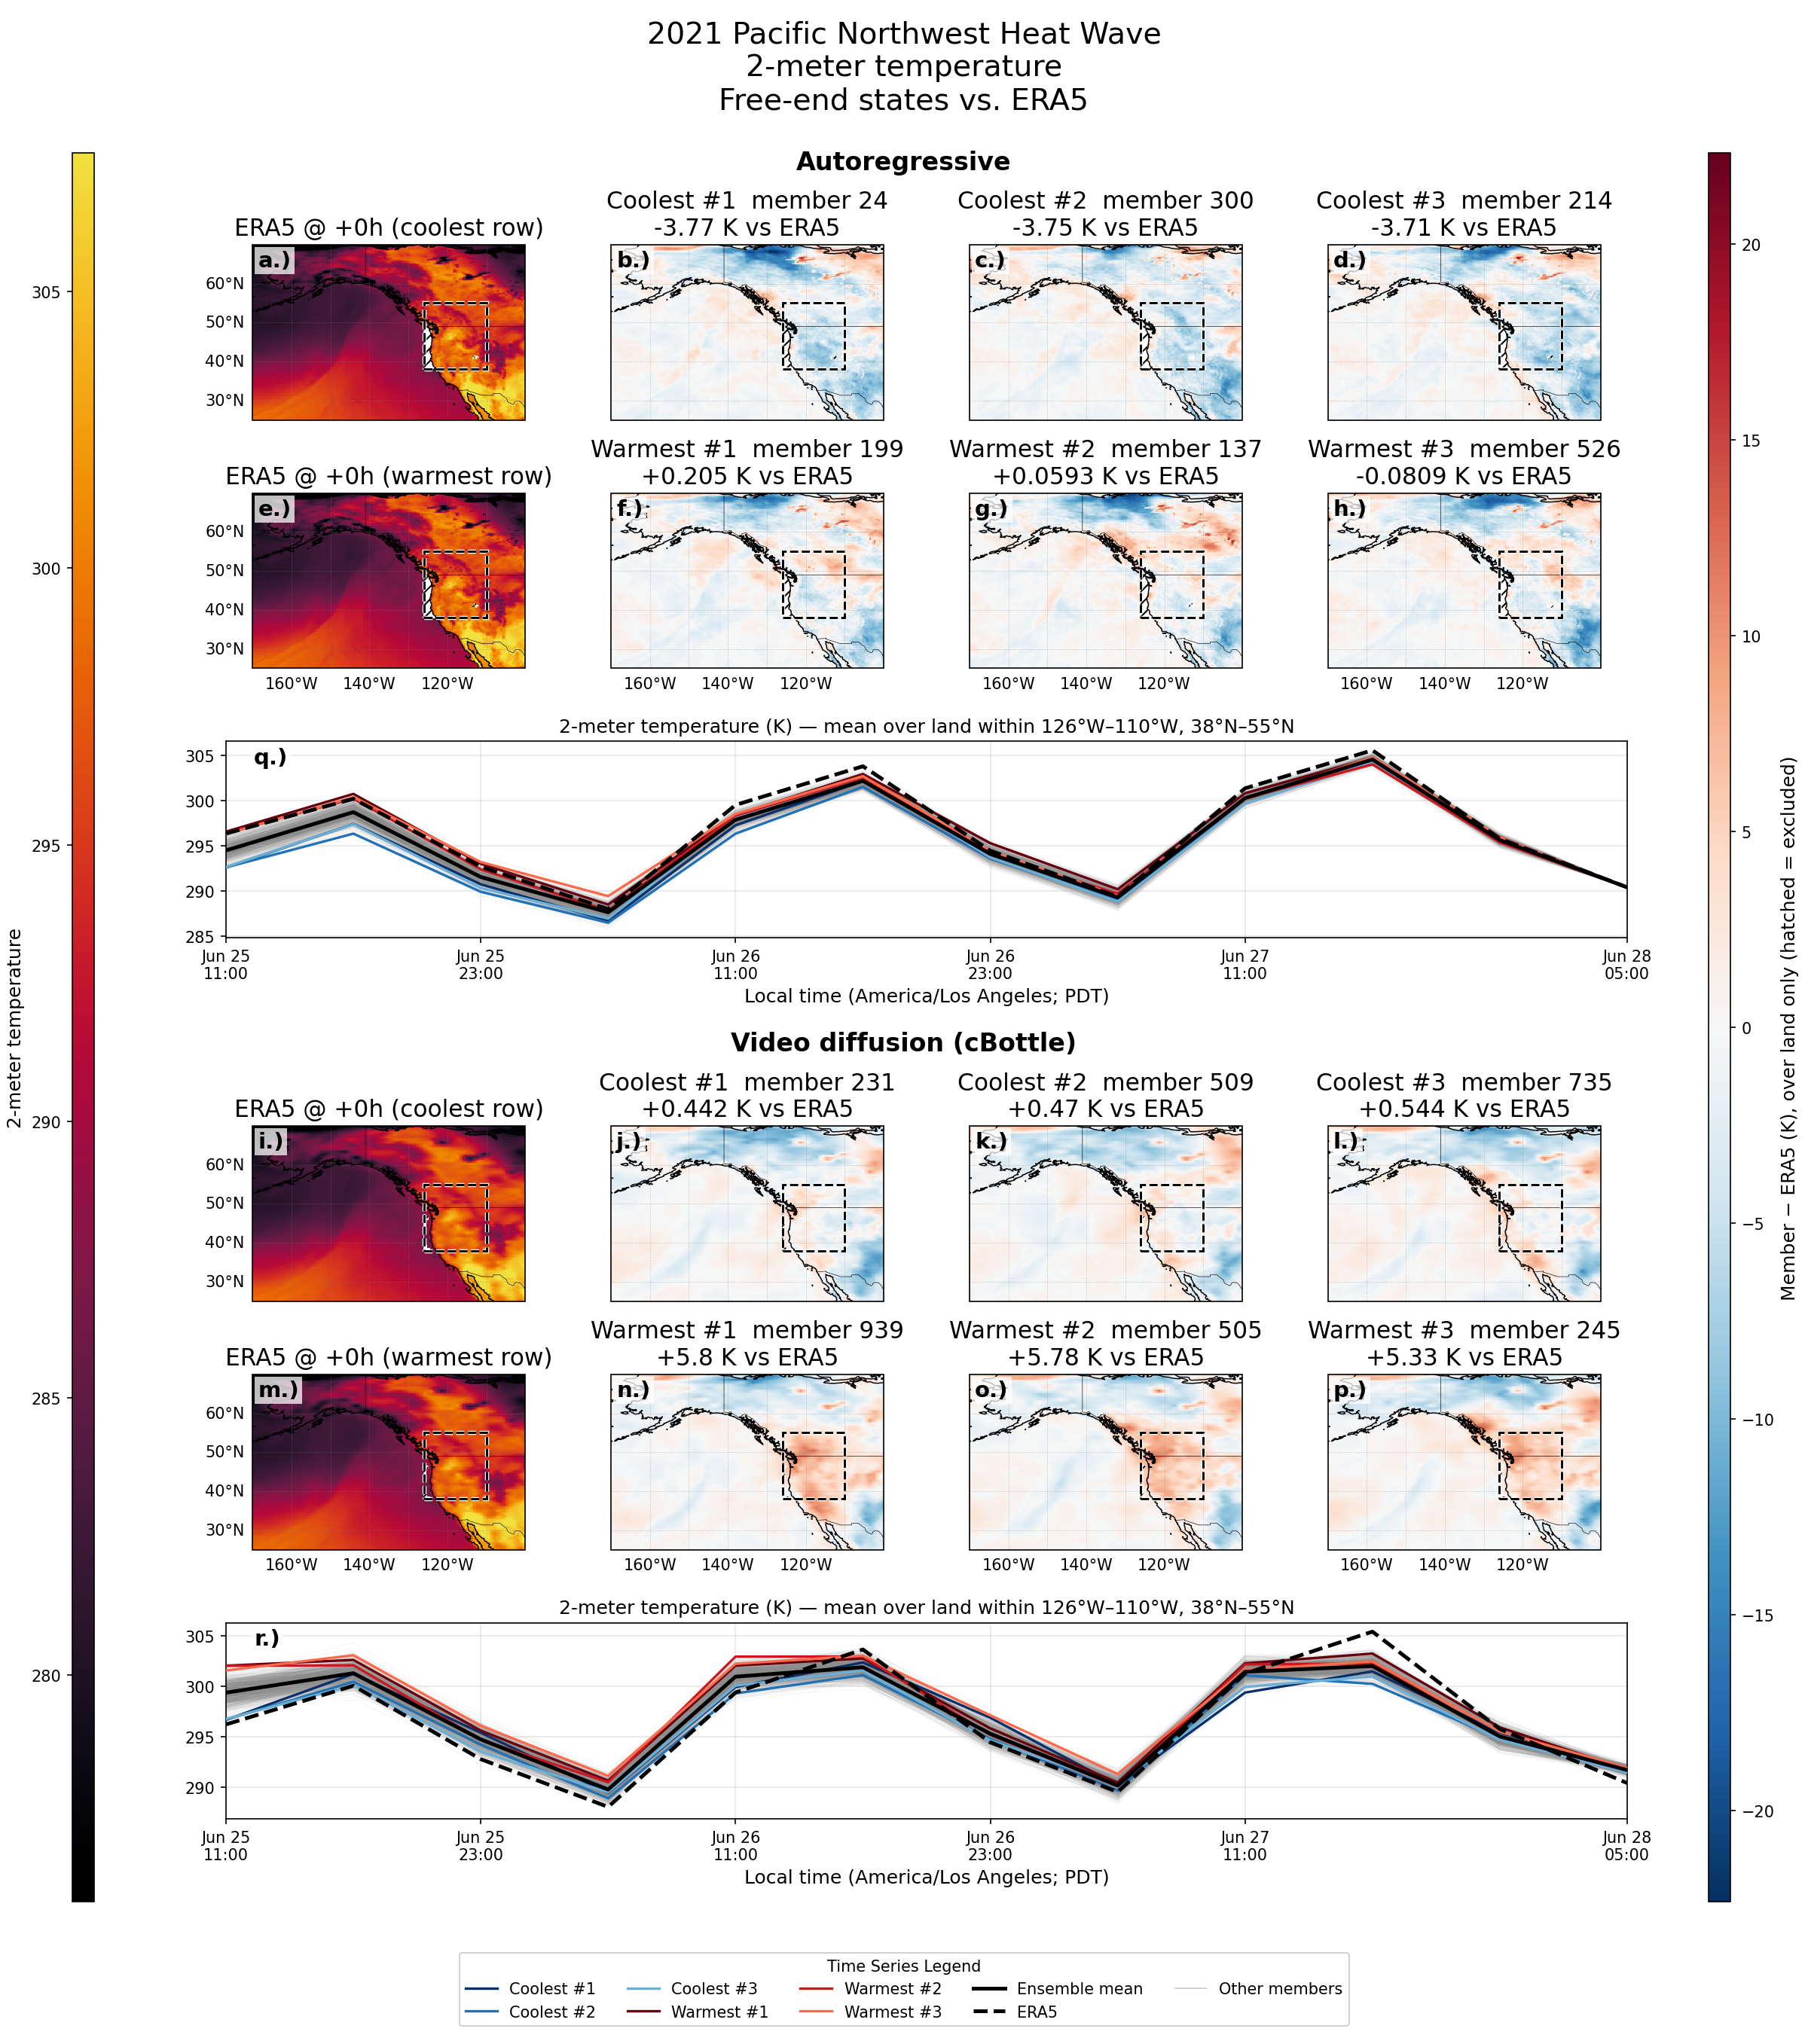
\includegraphics[width=\linewidth]{free_end_states_compare_pnw_heatwave.png}
  \caption{Pacific Northwest heatwave 66-hour end-conditioned ensemble comparison between the autoregressive model and cBottle-video. (a--h) Free-end ($t=0$, June 25, 11:00 PDT) 2-meter temperature ($t_{2\text{m}}$) states and anomalies relative to ERA5 for the autoregressive model, showing the three coolest (b--d) and three warmest (f--h) ensemble members averaged over land within $126^\circ$--$110^\circ$~W and $38^\circ$--$55^\circ$~N (dashed box). (i--p) As in (a--h), but for cBottle-video. (q,r) Evolution of land-mean $t_{2\text{m}}$ (K) over local time (PDT) across ensemble members for the autoregressive model and cBottle-video, respectively, with dashed black lines denoting ERA5 verification. The autoregressive ensemble retains 778 of its 1,000 members after stability screening.}
  \label{fig:pnw-free-end-states}
\end{figure}

Figure~\ref{fig:pnw-free-end-states} compares 66-hour end-conditioned ensemble trajectories ending at the heatwave peak (June 28, 2021, 12:00 UTC / 05:00 PDT) across the autoregressive model and cBottle-video. In cBottle-video, ensemble members begin uniformly warmer than ERA5 reanalysis at the free-end frame ($t=0$, June 25, 11:00 PDT), with the warmest members exceeding ERA5 by up to $+5.8$\,K over land (Figure~\ref{fig:pnw-free-end-states}j--p). Throughout the 66-hour interval, these diffusion members' temperature remains persistently elevated, failing to capture the observed day-over-day warming and intensification leading into the June 27 peak (Figure~\ref{fig:pnw-free-end-states}r).

In contrast, the autoregressive model generates antecedent states that begin cooler and closely bracket reanalysis (coolest member $-3.77$\,K vs.\ ERA5, warmest $+0.20$\,K vs.\ ERA5; Figure~\ref{fig:pnw-free-end-states}b--h). As time progresses toward the pinned extreme, the autoregressive ensemble ($N=778$ stable members) faithfully captures the progressive diurnal building and multi-day intensification culminating in the June 27 peak (Figure~\ref{fig:pnw-free-end-states}q).

Furthermore, antecedent surface temperatures in the autoregressive ensemble are more strongly associated with the large-scale height field---an expected finding given the central role of the blocking high in driving the heatwave. An EOF analysis of the free-end $z_{500}$ anomaly field ($170^\circ$--$100^\circ$~W, $25^\circ$--$70^\circ$~N) reveals that the leading eight principal components explain 17\% of across-member land-mean $t_{2\text{m}}$ variance in-sample and 15\% under 10-fold cross-validation (within-model in-sample OLS F-test, $p < 0.001$; Supplementary Figure~\ref{fig:pnw-eof-regression}b). By contrast, the leading eight modes computed separately for cBottle-video explain 9\% in-sample ($R^2_{\text{CV}} = 0.08$; Supplementary Figure~\ref{fig:pnw-eof-regression}c).



\section{Discussion and conclusion}

Backward autoregression learns the conditional antecedent distribution $p(\mathbf{x}_{t-\Delta t}\mid\mathbf{x}_t)$ rather than reversing physics, as coarse-graining suppresses the high-wavenumber dissipation that would otherwise make reversal impossible \citep{Hassanzadeh2026-dd}. Within the 66-hour window, our trajectories appear more physically credible than those from cBottle-video, although numerical stability screening already excludes 13.3\% of Ian and 22.2\% of Pacific Northwest members by 66 hours. Improving stability and increasing training volume are clear next steps toward supporting locality-specific climate-risk assessments without massive forward ensembles.

\section*{Code Availability}
The code used to train the backward-in-time FourCastNet~3 model is available at
\url{https://github.com/jerrylin96/run-it-back}. Scripts used to compare the
model with cBottle-video are available at
\url{https://github.com/jerrylin96/rewinding-the-extremes/tree/main/scripts/backward_emulator}.

\section*{Author Contributions}
Jerry Lin: Software, Conceptualization, Writing -- original draft, Writing --
review and editing. Elizabeth A. Barnes: Supervision, Funding acquisition,
Conceptualization, Writing -- review and editing.

\begin{ack}
J.L. was supported by the U.S. Department of Energy Office of Science through
the Program for Climate Model Diagnosis and Intercomparison (PCMDI).
\end{ack}

\section*{Use of Generative AI and AI-Assisted Technologies}
Claude Fable 5.1, Fable 5, and Claude Opus 4.8, accessed through Claude Code Web, were used to edit code and text, assist with literature searches, and draft the initial
Supporting Information. GPT-5.6 Sol in OpenAI Codex was used for adversarial
code review. GPT-5.6 Sol in OpenAI Prism and Gemini 3.8 Flash in Antigravity
CLI were used to revise text for flow and clarity. Arena.ai was used to refine
overly complex sentences. GPT-6 Luna in OpenAI Prism was used to prepare these
camera-ready statements and edit the manuscript's LaTeX front matter. The
authors reviewed and verified the AI-assisted material and take responsibility
for the final manuscript.

\clearpage

{\small
\bibliographystyle{unsrtnat}
\bibliography{references}
}

\clearpage
\appendix
\section{Supplementary information}

\setcounter{figure}{0}
\renewcommand{\thefigure}{S\arabic{figure}}
\renewcommand{\theHfigure}{S\arabic{figure}}

\begin{figure}[ht]
  \centering
  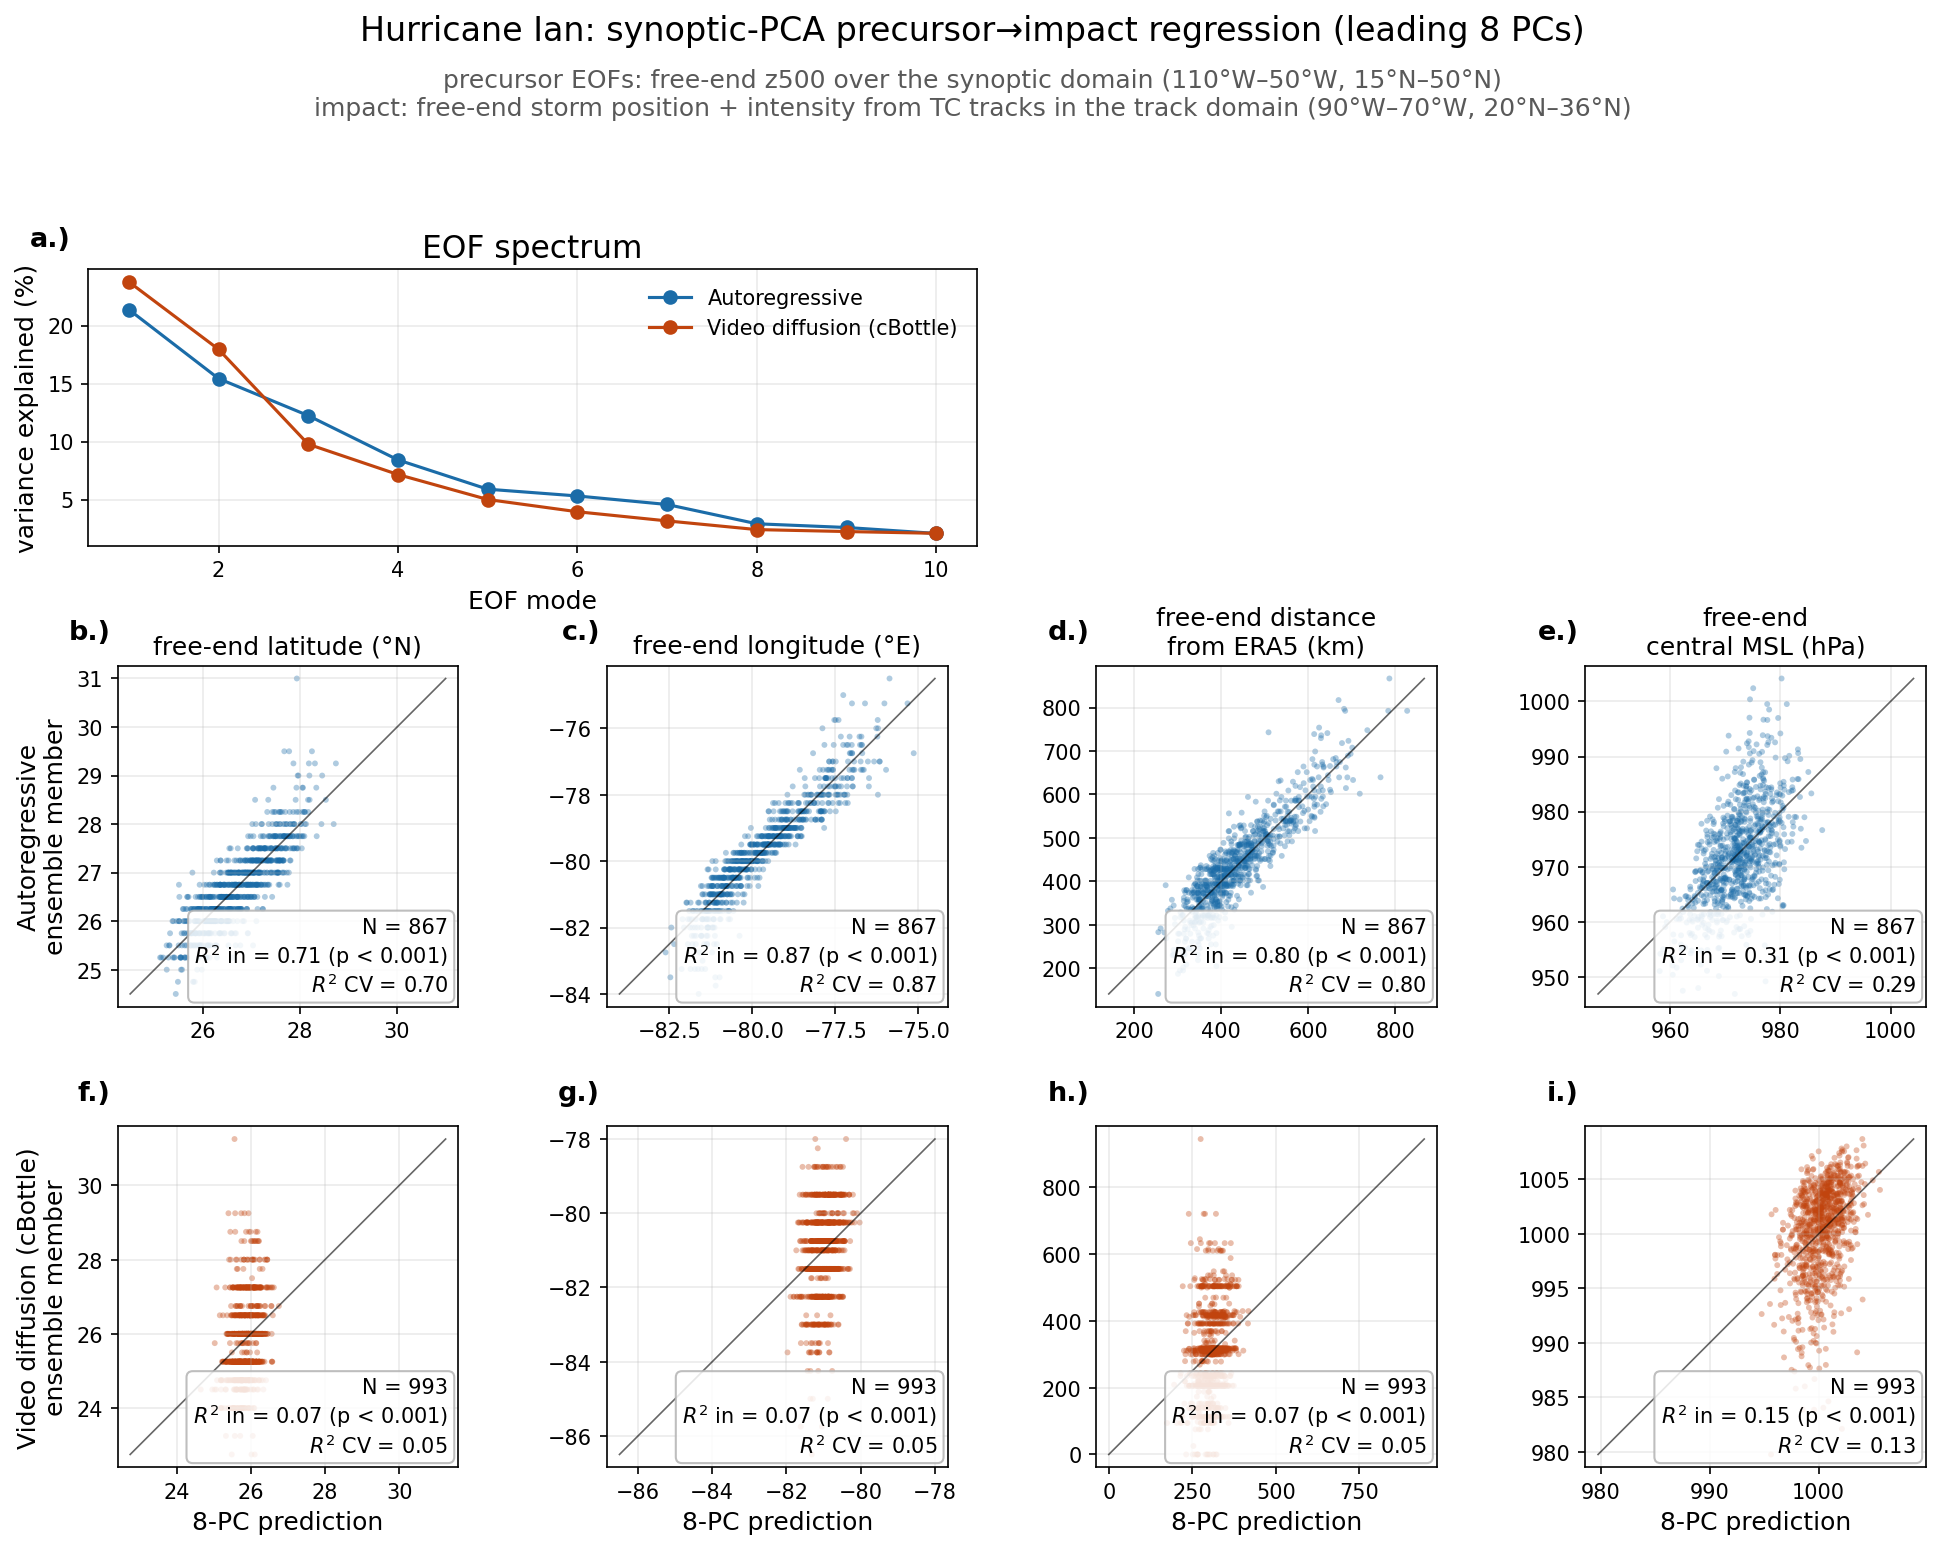
\includegraphics[width=\linewidth]{eof_regression_ian.png}
  \caption{Hurricane Ian free-end synoptic EOF and regression diagnostics. (a) Variance explained by the leading EOFs of $z_{500}$ over $110^\circ$--$50^\circ$~W and $15^\circ$--$50^\circ$~N. (b--e) Autoregressive ensemble-member values versus predictions from regressions on that ensemble's leading eight principal components for storm latitude, longitude, distance from ERA5, and minimum mean sea level pressure, respectively. (f--i) As in (b--e), using cBottle-video's own leading eight principal components. Insets report in-sample/CV coefficients of determination; gray lines denote one-to-one agreement.}
  \label{fig:si-eof-regression-ian}
\end{figure}

\begin{figure}[t]
  \centering
  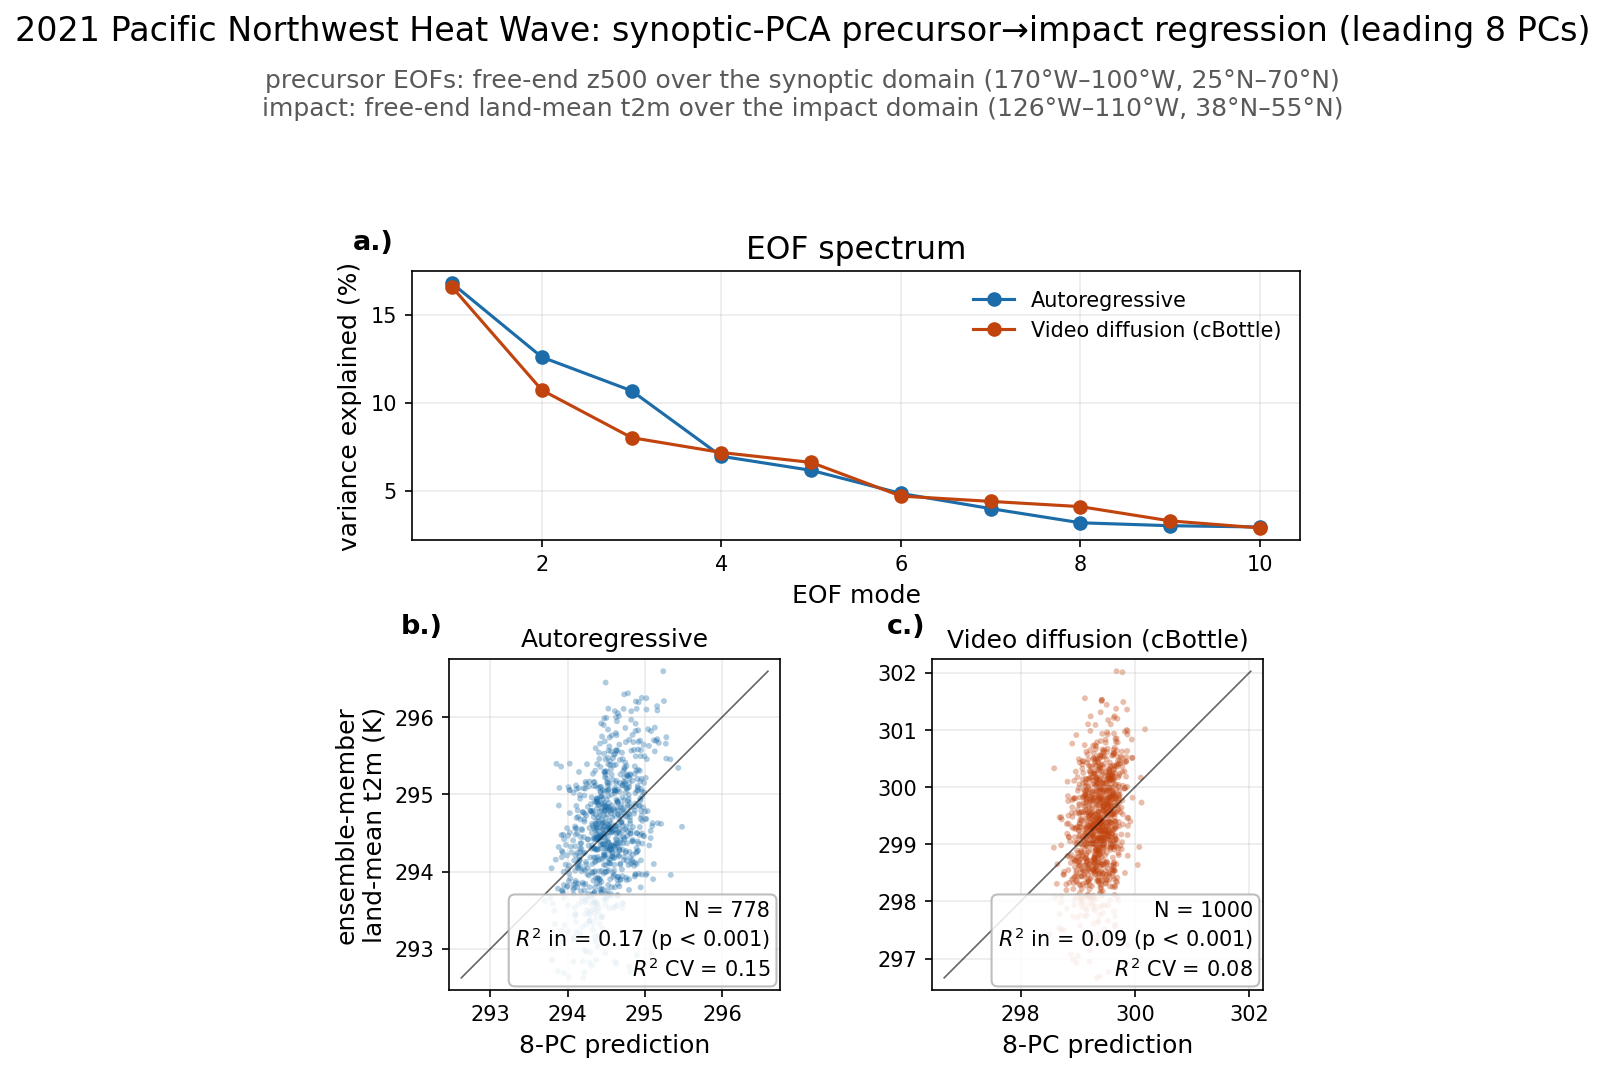
\includegraphics[width=\linewidth]{eof_regression_pnw_heatwave.png}
  \caption{Pacific Northwest heatwave free-end synoptic EOF and regression diagnostics. (a) Variance explained by the leading EOFs of $z_{500}$ over $170^\circ$--$100^\circ$~W and $25^\circ$--$70^\circ$~N. (b,c) Ensemble-member land-mean 2-m temperature over $126^\circ$--$110^\circ$~W and $38^\circ$--$55^\circ$~N versus predictions from regressions on each ensemble's own leading eight principal components for the autoregressive and cBottle-video ensembles, respectively. Insets report in-sample/CV coefficients of determination; gray lines denote one-to-one agreement.}
  \label{fig:pnw-eof-regression}
\end{figure}

\subsection{Case-study ensemble screening and regression diagnostics}

Each case and model started with 1,000 members. The autoregressive ensembles retain 867 Ian members and 778 Pacific Northwest members after numerical stability screening; at 66 hours, these screens exclude 13.3\% and 22.2\% of the respective ensembles. The screen rejects a member when its global $t_{2\text{m}}$ field is nonfinite or contains values outside $[150,350]$\,K, and carries the failure through the remaining backward rollout. All 1,000 autoregressive Ian members pass track quality control. cBottle-video retains 993 Ian members after track quality control; seven lack a qualifying Ian track.

For each case and model, the EOF basis is computed separately from that ensemble's free-end $z_{500}$ anomalies. The leading eight ensemble-derived principal components are fixed for 10-fold cross-validation: OLS is refit in each fold, but PCA is not. Reported $p$-values are within-model in-sample OLS F-tests and do not test differences between models.

\clearpage

\subsection{Backward-in-time probabilistic autoregressive model}
\label{sec:methods_fcn3_backward}

\paragraph{Formulation and backbone architecture.}
To reconstruct antecedent atmospheric states, we formulate a single-step backward autoregressive model $f_\theta: \mathbf{x}_t \mapsto \mathbf{x}_{t - \Delta t}$ with time step $\Delta t
  = 6\,\text{h}$. Because forward atmospheric dissipation renders the time-reversed mapping inherently one-to-many, deterministic regression collapses unresolvable fine scales
  toward a blurry conditional mean. We therefore employ the FourCastNet~3 (FCN3) architecture configured as a probabilistic ensemble model. The model backbone consists of a 10-layer spherical neural operator (273,507,540 real scalar parameters, counting each complex weight as two real scalars; approximately $273.5\times 10^6$ parameters, latent width $d=384$, latent spatial downsampling factor of $2$) in which each block combines a pointwise MLP with a spherical convolution---local discrete-continuous (DISCO) convolutions in most blocks, and a global spectral convolution (in the manner of SFNO) in the first block of every five (2 of 10 blocks).

\paragraph{State representation and auxiliary conditioning.}
The prognostic atmospheric state $\mathbf{x}_t \in \mathbb{R}^{72 \times 721 \times 1440}$ is defined on a $0.25^\circ$ equiangular grid from ERA5 reanalysis, comprising 72 vertical and surface channels: 5 upper-air fields ($u, v, z, T, q$) across 13 pressure levels (50--1000\,hPa) and 7 surface fields ($u_{10\text{m}}, v_{10\text{m}}, u_{100\text{m}}, v_{100\text{m}}, t_{2\text{m}}, \text{MSL}, \text{TCWV}$). Static and dynamic auxiliary inputs are mapped through a dedicated auxiliary encoder ($d_{\text{aux}}=36$): surface geopotential ($Z$), land-sea mask ($\text{LSM}$), input-aligned top-of-atmosphere solar zenith angle $\cos\theta_z(t)$, and 8 multi-scale, spatially correlated spherical diffusion noise channels ($k_T \in [3.08\times 10^{-5}, 5.05\times 10^{-1}]$). Wind vector components $(u, v)$ are normalized via wind-angle-aware standardization (shared variance per level based on total horizontal wind magnitude), moisture fields ($q, \text{TCWV}$) are min-max scaled with a non-negative output clamp, and all remaining fields use standard $z$-score normalization.

\paragraph{Objective and training setup.}
The model is trained on 10 years of ERA5 reanalysis (2009--2018; validated on 2019) using an ensemble continuous ranked probability score (standard CDF-based CRPS) with a spectral penalty:
\begin{equation}
\mathcal{L} = \sum_{c=1}^{72} w_c \left[ \mathcal{L}_{\text{CRPS}}\!\left(\hat{\mathbf{x}}_{t-\Delta t}^{(c)}, \mathbf{x}_{t-\Delta t}^{(c)}\right) + 0.1\,
\mathcal{L}_{\text{Spectral-CRPS}}\!\left(\hat{\mathbf{x}}_{t-\Delta t}^{(c)}, \mathbf{x}_{t-\Delta t}^{(c)}\right) \right],
\end{equation}
where the raw channel weights $a_c$ are $0.1$ for surface fields, $a_{t_{2\text{m}}} = 1.0$, and $a_c = 0.001 \times p\,[\text{hPa}]$ for atmospheric pressure levels, and $w_c = a_c / \sum_j a_j$ are their normalized values. Both loss terms additionally include the channelwise factor $s_c / \max(\sigma_{\Delta x,c}, 10^{-4})$, where $s_c$ is the state-normalization scale and $\sigma_{\Delta x,c}$ is the six-hour tendency standard deviation; this factor may be absorbed into the loss terms, so final effective multipliers need not sum to one. Spectral-CRPS is CRPS on magnitudes of spherical-harmonic coefficients. Optimization uses Adam ($\text{lr} = 5\times 10^{-4}$, $\beta_1 = 0.9, \beta_2 = 0.95$, gradient clipping norm $16$,
global batch size $4$, training ensemble size $E=8$) with a \texttt{ReduceLROnPlateau} scheduler. Multistep backward rollouts are computed autoregressively: step $k$ predicts $\hat{\mathbf{x}}_{t-(k+1)\Delta t}$ from $\hat{\mathbf{x}}_{t-k\Delta t}$ conditioned on $\cos\theta_z(t-k\Delta t)$ with an autoregressively updated diffusion noise state.

Parameters were optimized on ERA5 from 2009--2018, with 2019 used for validation. State-normalization and six-hour tendency statistics were computed over 1979--2018 and reused unchanged. We evaluated the epoch-14 checkpoint (iteration 51,128), selected by minimum validation loss for the combined CRPS and spectral-CRPS objective. Training used BF16 mixed precision; case-study rollouts used FP32 with TF32 disabled.

\subsection{cBottle-video}
\label{sec:methods_cbottle}

\paragraph{Architecture and spherical grid discretization.}
cBottle-video \citep{Brenowitz2025-mz} employs a continuous-time score-based diffusion model using an adapted Song-UNet architecture \citep{Song2020-hs, Karras2022-xq}. The network incorporates learned position embeddings, diurnal and seasonal time embeddings, AMIP mid-month SST boundary conditions linearly interpolated to each
frame's valid time, and temporal self-attention layers across frames \citep{Ho2022-lf, Blattmann2023-zo}. To circumvent spherical distortion and pole singularities in conventional latitude-longitude grids, the model operates on an equal-area HEALPix (HPX64) spherical discretization with custom face padding \citep{Karlbauer2024-nv}. HPX64 partitions the globe into 12 square faces of $64 \times 64 = 4{,}096$ pixels (49,152 total pixels globally), yielding an effective spatial resolution of $\sim$100\,km.

\paragraph{Masked video diffusion and score-based sampling.}
Training employs a masked-conditional video diffusion (MCVD) framework \citep{voleti2022MCVD} over 66-hour sequences (12 frames at $\Delta t = 6\,\text{h}$). During training, stochastic masking patterns (random frame dropout, block-wise masking, endpoint interpolation, and unconditional masking) enable arbitrary temporal inpainting
\citep{Brenowitz2025-mz}. The schematic denoising component of the training objective is:
\begin{equation}
\label{eq:cbottle_training_objective}
\begin{aligned}
\min_{\theta}\; &\mathbb{E}_{\mathbf{x},m,\sigma,\epsilon}\left[\lambda(\sigma)
\left\|\mathcal{D}_\theta(\mathbf{x} + \epsilon; \sigma, \mathbf{c}_m) - \mathbf{x}\right\|^2\right],\\
&\lambda(\sigma) = \frac{\sigma^2 + \sigma_{\text{data}}^2}{(\sigma\sigma_{\text{data}})^2},
\qquad \epsilon \sim \mathcal{N}(0, \sigma^2 \mathbf{I}),
\end{aligned}
\end{equation}
where $\mathbf{c}_m$ denotes the temporal-mask and auxiliary conditioning associated with mask $m$; the expression suppresses valid-channel masking and reductions. The referenced public training caller uses $\sigma_{\text{data}} = 1.0$, and its video recipe samples $\sigma$ log-uniformly over $[0.02, 1000]$. We evaluate a single public cBottle-video denoiser at all sampling noise levels; no noise-dependent expert switching is used. Samples are drawn across 18 discretization steps by integrating the reverse-time probability-flow ODE:
\begin{equation}
\label{eq:cbottle_sampling_step}
\frac{d\mathbf{x}}{d\sigma} = \frac{\mathbf{x} - \mathcal{D}_\theta(\mathbf{x}, \sigma)}{\sigma}
\end{equation}
using the deterministic second-order Heun sampler of \citet{Karras2022-xq} with $S_{\text{churn}} = 0$.

\paragraph{Conditioning and inference setup.}
We evaluate the public pre-trained checkpoint \citep{Brenowitz2025-mz} via \texttt{Earth2Studio} \citep{Earth2Studio_Contributors_NVIDIA_Earth2Studio_2024}, implementing
flexible masked conditioning by subclassing its inference wrapper. Conditioning frames are extracted from $0.25^\circ$ ERA5 reanalysis \citep{Hersbach2020-oh} and regridded to HPX64. For Hurricane Ian, $t=0$ is September 28, 2022, 00:00 UTC, and $t=66\,\text{h}$ is September 30, 2022, 18:00 UTC. ERA5 at $t=66\,\text{h}$ supplies final-frame conditioning, and the sampler jointly generates all 12 frames without overwriting its generated endpoint with ERA5, for each of the 1,000 ensemble members.



\end{document}